\documentclass[10pt,twoside,cucitura,classica,english,openany]{toptesi}

\usepackage{hyperref}
\hypersetup{%
  pdfpagemode={UseOutlines},
  bookmarksopen,
  pdfstartview={FitH},
  colorlinks,
  linkcolor={blue},
  citecolor={red},
  urlcolor={blue}
}
\usepackage[latin1]{inputenc}
\usepackage[T1]{fontenc}\usepackage{lmodern}
\usepackage{layaureo}
\usepackage{amsmath}
\usepackage{amssymb}
\usepackage{placeins}
\usepackage[titletoc]{appendix}
\usepackage[font=footnotesize]{caption}
\usepackage[font=footnotesize]{subcaption}
\usepackage[style=numeric, sorting=none, backend=biber]{biblatex}
\addbibresource{references.bib}

\bibliography{bibliography}

\ateneo{Stockholm University}
\facolta{Department of Physics}

\titolo{Search for in Mono-jet Final States with the ATLAS Experiment}

\TesiDiLaurea{Licensiate Thesis}

\CorsoDiLaureaIn{Doctoral Studies in }
\corsodilaurea{Physics}

\CandidateName{Candidate:}
\candidato{Gabriele \textsc{Bertoli}}
\AdvisorName{Advisor:}
\relatore{dott.~Christophe \textsc{Clement}}
\CoAdvisorName{Co-Supervisor}
\secondorelatore{dott.~David \textsc{Milstead}}
\sedutadilaurea{December 2015}
\sedutadilaurea{\textsc{December 12,} 2015}
\logosede{logo}

\newtheorem{osservazione}{Osservazione}
\ExtendCaptions{english}{Abstract}{Acknowledgments}

\graphicspath{{images/}}

\begin{document}\errorcontextlines=9

\numberwithin{equation}{section}

\newcommand*{\parder}[2]{\displaystyle\frac{\partial #1}{\partial #2}}
\newcommand*{\ud}{\mathrm{d}}
\newcommand*{\er}{e_{R}}
\newcommand*{\el}{e_{L}}
\newcommand*{\eplus}{e^{+}}
\newcommand*{\eminus}{e^{-}}
\newcommand*{\vect}[1]{\overrightarrow{#1}}
\newcommand*{\bra}[1]{\langle #1|}
\newcommand*{\ket}[1]{|#1\rangle}
\newcommand*{\MET}{\mbox{$E\kern-0.50em\raise0.10ex\hbox{/}_{T}$}}
\newcommand*{\met}{E_\mathrm{\, T}^\mathrm{\, miss}}
\newcommand*{\et}{E_\mathrm{\, T}}
\newcommand*{\pt}{p_\mathrm{\, T}}
\newcommand*{\ifb}{\mbox{fb$^{-1}$}}
\newcommand*{\zee}{Z \to e e}
%%% Local Variables:
%%% mode: latex
%%% TeX-master: "main"
%%% End:


\english

\cleardoublepage

% \expandafter\ifx\csname StileTrieste\endcsname\relax
\frontespizio
% \else
\paginavuota
\begin{dedica}
\end{dedica}
% \tomo \fi

\ringraziamenti

\tablespagetrue\figurespagetrue \indici

% \expandafter\ifx\csname StileTrieste\endcsname\relax \else
\begin{citazioni}
  \textit{Si sta,\\come d'autunno,\\sugli alberi,\\le foglie }

  [\textsc{G.~Ungaretti}, Soldati]
\end{citazioni}

% \fi

\chapter*{Introduction}
\label{cha:intro}
The Standard Model of particle physics is the theory used to describe the
elementary constituents of matter and their interactions. Through the years is
has been tested by many experiments and despite its success it cannot explain,
among other problems, the so called hierarchy and dark matter problems described
in \cref{cha:beyond-stand-model}. Supersymmetry is an extension of the Standard
Model that could solve these issues by introducing new particles. The lightest
of these particles, the so called neutralino (and denoted by
$\widetilde{\chi}_{\, 1}^{\, 0}$), in the context of a minimal supersymmetric
model, could be produced in squark pair production with $\squarkprod$ and,
lacking electromagnetic and strong interaction~\cite{MSSMIntro}, escape
detection. With an energy in the center of mass of $\sqrt{s} = 13$~TeV, the
\gls{lhc} could be able to produce such kind of particles, the ATLAS detector
could be able to infer their presence by the momentum unbalance they would
create. This thesis presents the result of the search for compressed
supersymmetric squark--neutralino signal with the ATLAS detector in the
3.2~$\ifb$ delivered in 2015 in an experimental signature with jets and large
missing transverse momentum in the final state.
%%% Local Variables:
%%% mode: latex
%%% TeX-master: "../search_for_DM_LED_with_ATLAS"
%%% End:


\mainmatter

\chapter{Theoretical overview}
\label{cha:theoretical-overview}

\section{The Standard Moldel of particle physics}
\label{sec:stand-mold-part}

The \gls{sm} is a theoretical model which describes the elementary constituents
of matter and their interactions. Up to now, we discovered three kind of
different interactions, the \emph{strong}, the \emph{electroweak} and the
\emph{gravitational}; excluding gravity, all of them are described by means of a
\emph{quantum field gauge theory}.

The Standard Model is the collection of these gauge theories, it is based on the
gauge symmetry group $SU(3)_C \times SU(2)_L \times U(1)_Y$ where $SU(3)_C$ is
the symmetry group of the \emph{Quantum Chromo-Dynamics} (QCD), the ``C''
subscript stands for \emph{color charge} which is the conserved charge in the
strong interaction. The $SU(2)_L$ is the weak isospin group acting on
\emph{left-handed} doublet of fermions while the $U(1)_Y$ group is the
\emph{hypercharge} symmetry group. Together $SU(2)_L \times U(1)_Y$ form the
electroweak symmetry group.

The Standard Model also contains and has predicted the existence of
\emph{elementary particles} that interacts between them via the forces mentioned
above. The matter constituents are called \emph{fermions}, the interaction are
mediated by other particles called \emph{gauge bosons}. Fermions are further
categorized into \emph{quark} which bound to form \emph{hadrons} and interact
through the strong force and \emph{leptons} which do not experience the strong
force. These are the true fundamental constituents of matter; the gauge bosons
arise from the gauge symmetry group of the Standard Model.

The existence of all the leptons, quarks and gauge bosons is confirmed by
experimental tests. Among the bosons, the Higgs boson is peculiar because,
unlike the others, it carries spin 0 and it is not associated with any
interaction, instead arises as a consequence of the \emph{spontaneously broken
  symmetry} of the electroweak sector which is the property, responsible of
giving mass to all the elementary particles and the weak gauge bosons.
%%% Local Variables:
%%% mode: latex
%%% TeX-master: "../search_for_DM_LED_with_ATLAS"
%%% End:


\section{The hierarchy problem and naturalness}
\label{sec:hier-probl-natur}

The \emph{naturalness criterion} states that one such [dimensionless and
measured in units of the cut-off] parameter is allowed to be much smaller than
unity only if setting it to zero increases the symmetry of the theory. If this
does not happen, the theory is unnatural~\cite{thooft:gauge}.

There are two important concepts in physics that enter in the formulation of the
naturalness principle, symmetries and effective field
theories. \emph{Symmetries} are closely connected to conservation laws, moreover
theory parameters that are protected by a symmetry, if smaller than the unit,
are not problematic according to the naturalness criterion. \emph{Effective
  field theories} are a sort of simplification of a more general theory that use
less parameters to describe the dynamics of particles with energies less than a
cut-off scale $\Lambda$.

Let us now consider the strength of the gravitational force, characterized by
the Newton's constant, G$_N$ and the weak force, characterized by the Fermi's
constant G$_F$, if we take the ratio of these we get:
\begin{equation}
  \label{eq:gf_gn_ratio}
  \frac{G_F \hbar^2}{G_N c^2} = 1.738 \times 10^{33}.
\end{equation}
The reason why this number is worth some attention is that theory parameters
close to the order of the unit in the SM, may be calculated in a more
fundamental theory, if any, using fundamental constants like $\pi$ or $e$ while
very big numbers may not have such a simple mathematical expression and thus may
lead to uncover new properties of the fundamental theory.

This number becomes even more interesting if we consider quantum effects.
\emph{Virtual particles} are not really particles but rather disturbances in a
field, these disturbances are off-shell ($E \neq m^2 + p^2$) and according to
the \emph{uncertainty principle}, $\Delta t \Delta E \geq \hbar / 2$, can appear
out of nothing for a short time that depends on the energy of the virtual
particle; according to quantum field theory, the vacuum is populated with such
disturbances. The Higgs field, has the property to couple with other SM
particles with a strength proportional to their mass. Now all these virtual
particles have a mass determined by the available energy $\Lambda$ and when the
Higgs field travels through space, it couples with these virtual particles and,
due to quantum corrections, its motion is affected and its invariant mass
squared gets a contribution proportional to $\Lambda$:
\begin{equation}
  \label{eq:delta_mh}
  \delta m_H^2 = k \Lambda^2 \text{, with } k = \frac{3 G_F}{4 \sqrt{2}
    \pi^2}(4m_t^2 - 2m_W^2 - m_Z^2 - m_H^2).
\end{equation}
Since $k \approx 10^{-2}$\cite{Giudice:2008bi}, the value of Higgs' mass
$m_H \sim G_F^{-1/2}$, should be close to the maximum energy scale $\Lambda$ and
if we assume this to be the Plank scale $M_{Pl} = G_N^{-1/2}$, the ration
$G_F/G_N$, should be close to the unity which contradicts
eq.~\eqref{eq:gf_gn_ratio}, this goes by the name of \emph{hierarchy problem}.

The large quantum corrections in~\eqref{eq:delta_mh} are mainly due to the fact
that in the SM, there is no symmetry protecting the mass of the Higgs'
field. Supersymmetry (SUSY), among other things, is capable of solving the
hierarchy problem by canceling out the quantum corrections that bring $m_H$
close to $\Lambda$ thus restoring the naturalness of the SM.
%%% Local Variables:
%%% mode: latex
%%% TeX-master: "../search_for_DM_LED_with_ATLAS"
%%% End:


\chapter{Experimental apparatus}
\label{cha:exper-appar}

\section{The large hadron collider}
\label{sec:large-hadr-coll}

The \gls{lhc}~\cite{LHC} is a two ring superconducting hadron accelerator and
collider located at the \gls{cern}.

The performance of a collider is evaluated in terms of its available
\emph{center of mass energy}, $\sqrt{s}$ and the \emph{instantaneous luminosity}
$\lumi$. The former defines the accessible energies for particle production. The
latter is defined as the interaction rate per unit cross section of the
colliding beams (collisions / (cm$^2$ s)).

The LHC is designed to operate at $\sqrt{s} = 14$~TeV in the center of mass
although it started off at 7~TeV in 2010 and 2011, 8~TeV in 2012 and 13~TeV in
2015 after the long shutdown in 2013 and 2014.

There are six experiments at LHC: ATLAS~\cite{ATLASPaper},
CMS~\cite{1748-0221-3-08-S08004}, ALICE~\cite{ALICE}, LHCb~\cite{LHCb},
LHCf~\cite{LHCf} and TOTEM~\cite{TOTEM}\@. ATLAS and CMS are designed to work
with the maximum luminosity that LHC can provide $\sim 10^{34}$~cm$^{-2}$
s$^{-1}$. This requirement, due to the low efficiency production, excludes the
use of anti-proton beams and therefore the LHC is designed to be a \gls{pp} and
heavy ions collider. The protons are organized in bunches, accelerated by LINAC2
to an energy of 50~MeV and subsequently injected in the \gls{psb}. Here they are
further accelerated to an energy of 1.4~GeV and fed to the \gls{ps} where they
reach the energy of 25~GeV to be then passed to the \gls{sps} which accelerate
them to an energy of 450~GeV. They are finally injected in the LHC in opposite
directions where they reach the nominal energy. There are four interaction
points where the four main experiments (ATLAS, CMS, ALICE, LHCb) are located, at
these locations, every 25~ns, the bunches cross and interact with each other
(\emph{bunch crossing}). A schematic view of the injection chain is depicted in
Figure~\ref{fig:lhc_inj_chain}.

The instantaneous luminosity depends on the beam parameters and is given by:
\begin{equation}
  \label{eq:54}
  \lumi = \frac{N^2_b n_b f_{rev} \gamma}{4 \pi \epsilon_n \beta^*} F
\end{equation}
where $N_b$ is the number of particles per bunch, $n_b$ is the number of bunches
per beam, $f_{rev}$ is the revolution frequency, $\gamma$ is the relativistic
gamma factor, $\epsilon_n$ the normalized transverse beam emittance, the beta
function is a measure of the transverse beam size and $\beta^*$ is the value of
the beta function at the interaction point and $F$ is the geometric reduction
factor due to the crossing angle of the beams at the \gls{ip}~\cite{LHC}. The
integrated luminosity is given by:
\begin{equation}
  \label{eq:55}
  L = \int \lumi \ud t
\end{equation}
and the integral is carried over data taking periods of the detector. The
integrated luminosity can be related to the total number of events of a certain
process by:
\begin{equation}
  \label{eq:56}
  N_{events} = L \sigma_{events}
\end{equation}
where $N_{events}$ is the total number of events, $L$ is the integrated
luminosity and $\sigma_{events}$ is the cross section for the process in units
of barn (1~b = 10$^{-28}$~m$^2$). In 2015 ATLAS recorded an integrated
luminosity of 3.2~\ifb.

\begin{figure}[!h]
  \centering
    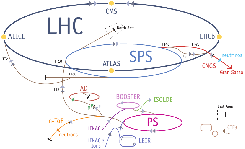
\includegraphics[width=.8\linewidth]{lhc_inj_chain}
    \caption{The LHC injection chain~\cite{LHCFAQ}.}
    \label{fig:lhc_inj_chain}
\end{figure}
%%% Local Variables:
%%% mode: latex
%%% TeX-master: "../search_for_DM_LED_with_ATLAS"
%%% End:


\section{The ATLAS detector}
\label{sec:atlas-detector}

\subsection{The inner detector}
\label{sec:inner-detector}

The inner detector (ID) is designed to provide good track reconstruction,
precise momentum resolution and both primary and secondary vertex measurements
above a nominal $\pt$ threshold of 0.5~GeV and within the pseudorapidity
$|\eta| < 2.5$. It also provides electron identification over $|\eta| < 2.0$ for
energies between 0.5~GeV and 150~GeV\cite{ATLASPaper}. The ID is 6.2~m long and
has a radius of about 1.1~m, it is surrounded by a solenoidal magnetic field of
2~T. Its layout is schematized in Figure~\ref{fig:id} and, as can be seen, it is
composed of three sub-detectors. At the inner radius the \emph{pixel detector}
mostly determines the position of primary and secondary vertex. The silicon
sensors are 250~$\mu$m thick detectors that operate with an initial bias voltage
of $\sim$150~V that will increase up to 600~V after 10 years of operation. In
the middle layer of the ID the \emph{semiconductor tracker} (SCT) is designed to
give eight precision measurements per track which contributes to the primary and
secondary vertex position and momentum measurements. The silicon sensors are 285
$\pm 15 \mu$m thick and initially operated with a bias voltage of $\sim$150
position
\begin{figure}[!h]
  \centering
    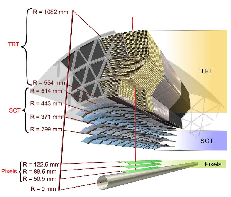
\includegraphics[width=.5\linewidth]{inner_detector}
    \caption{Schematic view of a charged track of 10~GeV $\pt$ that traverses
      the different ID sub-detectors. After traversing the beryllium pipe, the
      track passes through the three cylindrical silicon-pixel layers, the four
      layers of silicon-microstrip sensors (SCT) and the approximately 36 straws
      contained in the TRT within their support structure.}
    \label{fig:id}
\end{figure}
%%% Local Variables:
%%% mode: latex
%%% TeX-master: "../search_for_DM_LED_with_ATLAS"
%%% End:


\subsection{The calorimeters}
\label{sec:calorimeters}

The main purpose of a calorimeter is to measure the energy of electrons, photons
and hadrons by mean of materials capable of completely absorb the energy of the
incoming particles transforming it in some measurable quantity. Calorimeters can
be classified in two categories, \gls{em} and \emph{hadronic} depending on the
particle they are designed to detect. The EM calorimeters are mainly used to
detect photons and electrons while the task of hadronic calorimeters is to
identify hadrons. Both types of calorimeters can be further divided into
\emph{sampling calorimeters} and \emph{homogeneous calorimeters}. Sampling
calorimeters alternates layers of a dense material used to absorb the energy of
incident particles (absorber) and an active material to collect the signal. The
interaction between the particles and the absorber produces a shower of
secondary particles with progressively degraded energy which is deposited in the
active material in form of charge or light that can be converted into
energy. Homogeneous calorimeters use only one material that serves both as an
absorber and an active material~\cite{Calorimetry}.

The ATLAS calorimeter is a sampling calorimeter covering up the $|\eta| < 4.9$
region the large $\eta$ coverage, ensures a good missing transverse momentum
measurement (see Section~\ref{sec:miss-transv-energy}); an illustration of the
system is shown in Figure~\ref{fig:calo}.

The EM calorimeter has a barrel and two end-caps, covering the $|\eta| < 1.475$
and $1.375 < |\eta| < 3.2$ region respectively. It uses \gls{lar} as active
material and lead as absorber in an accordion geometry that provides $\phi$
symmetry without azimuthal cracks. In the region $|\eta| < 1.8$ a presampler
consisting of a LAr active region is used to correct for electrons and photons
energy loss upstream of the calorimeter.

There are then three hadronic calorimeters: the \gls{tilecal}, the \gls{hec} and
the \gls{fcal}. The TileCal barrel and extended barrels cover the $|\eta| < 1.0$
and $0.8 < |\eta| < 1.7$ and uses steel as absorber and scintillating tiles
connected to photomultipliers tubes through wavelength shifting fibers for
readout as an active material. The HEC covers the $1.5 < |\eta| < 3.2$ region
and, to avoid drops in material density at the transition, it overlaps slightly
with the FCal that covers the $3.1 < |\eta| < 4.9$.

\begin{figure}[!h]
  \centering
    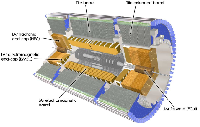
\includegraphics[width=.5\linewidth]{calorimeters}
    \caption{Cut-away view of the ATLAS calorimeter system.}
    \label{fig:calo}
\end{figure}
%%% Local Variables:
%%% mode: latex
%%% TeX-master: "../search_for_DM_LED_with_ATLAS"
%%% End:


\subsection{The muon spectrometer}
\label{sec:muon-spectrometer}

Insert this part
%%% Local Variables:
%%% mode: latex
%%% TeX-master: "../search_for_DM_LED_with_ATLAS"
%%% End:


\chapter{Physical objects reconstruction}
\label{cha:phys-objects-reconst}

\section{Lepton reconstruction and identification}
\label{sec:lept-reconstr-ident}

Object reconstruction is the process that associates the signal left in the
detector by charged particles to physical objects through a series of
algorithms. This analysis uses electrons, muons, jets and missing transverse
momentum ($\met$). Two types of electrons, muons and jets are also defined:
\emph{baseline} and \emph{good}, where the former one is used for removal of
overlapping objects and preselection while the latter for selecting the objects
used to define the signal and control regions. In the following a brief
introduction to the identification criteria of these objects is presented.
%%% Local Variables:
%%% mode: latex
%%% TeX-master: "../search_for_DM_LED_with_ATLAS"
%%% End:


\subsection{Electrons}
\label{sec:electrons}

Electrons are identified in the central part of the ATLAS detector
($|\eta| < 2.47$) by an energy deposit in the electromagnetic calorimeter and an
associated track in the inner detector. Electron identification efficiencies are
measured in $pp$ collisions data and compared to efficiencies measured in $\zee$
simulations. Signal electrons are identified by different sets of
likelihood-based criteria with $\sim 95\%, \sim 90\%$ and $\sim 80\%$ efficiency
for electrons with $\pt \sim 40~$GeV, the different criteria are referred to as
\emph{loose}, \emph{medium} and \emph{tight} operating points
respectively\cite{ATL-EL-IDENT}.
%%% Local Variables:
%%% mode: latex
%%% TeX-master: "../search_for_DM_LED_with_ATLAS"
%%% End:


\chapter{The Monojet signature}
\label{cha:monojet-signature}

\section{Motivation}
\label{sec:motivation}

There are two possible cases that results in an energy imbalance in the
detector, the first one occurs in beyond Standard Model physics, that involves
the presence of particles that interact weakly or not at all with normal
matter. These particles are not detected thus leaving an energy imbalance in the
detector. In the second case, the decay products in the final state involve
neutrinos that are not detectable by ATLAS\@. To better understand the category
category of events, consider \cref{fig:susy_standard} that shows the decay
topology of squark pair production with a neutralino and two jets in the final
state. Using the two body decay energy and momentum relations~\cite{PDG}:
\begin{equation}
  \label{eq:93}
  E_q = \frac{M_{\, \tilde{q}}^2 - m_{\, \tilde{\chi}_{\, 1}^{\, 0}}^2 + m_q^2}{2
    M_{\, \tilde{q}}},
\end{equation}
\begin{equation}
  \label{eq:94}
  |\vec{p}_q| = |\vec{p}_{\, \tilde{\chi}_{\, 1}^{\, 0}}| = \frac{\left[ \left(
        M_{\, \tilde{q}}^2 - (m_q + m_{\, \tilde{\chi}_{\, 1}^{\, 0}})^2
      \right) \left( M_{\, \tilde{q}}^2 - (m_q - m_{\, \tilde{\chi}_{\, 1}^{\,
            0}})^2 \right) \right]^{1/2}}{2 M_{\, \tilde{q}}}
\end{equation}
where $M_{\, \tilde{q}}$ is the squark center of mass energy,
$m_{\, \tilde{\chi}_{\, 1}^{\, 0}}$ is the neutralino mass and $m_q$ is the
quark mass. Neglecting the quark mass ($m_q = 0$) we get that:
\begin{equation}
  \label{eq:95}
  E_q = \frac{M_{\, \tilde{q}}^2 - m_{\, \tilde{\chi}_{\, 1}^{\, 0}}^2}{2 M_{\,
      \tilde{q}}},
\end{equation}
\begin{equation}
  \label{eq:96}
  |\vec{p}_q| = |\vec{p}_{\, \tilde{\chi}_{\, 1}^{\, 0}}| = \frac{M_{\,
      \tilde{q}}^2 - m_{\, \tilde{\chi}_{\, 1}^{\, 0}}^2}{2 M_{\, \tilde{q}}}.
\end{equation}
The quark will hadronize in the calorimeter and give rise to a jet that can be
detected by the ATLAS detector only if $\pt > 20$~GeV. If for example the mass
of the squark is $M_{\, \tilde{q}} = 450$~GeV and the mass of the neutralino is
$m_{\, \tilde{\chi}_{\, 1}^{\, 0}} = 445$~GeV then it can be seen from
\cref{eq:96} that the quark and neutralino momenta are given by
$|\vec{p}_q|~=~|\vec{p}_{\, \tilde{\chi}_{\, 1}^{\, 0}}|~\simeq~5$~GeV. Since
the neutralino escape detection, this results in low $\met$ thus when the mass
of the neutralino approaches the mass of the quark this results in a low energy
jet and $\met$ that cannot be used to trigger and select the event by the ATLAS
detector. This means that there is no sensitivity to SUSY models with compressed
mass spectra (when the mass difference between the particles is small). This
problem applies to many channels of SUSY productions.



\cref{fig:susy_exclusion} shows this effect for the search for squark pair
production in the case of the squark decaying directly to a quark and a
neutralino through the mechanism illustrated in \cref{fig:susy_standard}. This
search uses a classical multijet + $\met$ analysis, it can be seen that there is
no sensitivity close to the diagonal (dashed line) in the region
$400~<~M_{\, \tilde{q}}~<~600$~GeV.

If an initial state radiation jet is present in the event, as depicted in
\cref{fig:susy_compressed}, the squark--squark system gets boosted in the
opposite direction thus increasing the momentum of the decay products and the
missing energy leading to a signature of a high $\pt$ jet on one side and
additional jets and $\met$ on the other side of the event.

Events with an energetic jet $\pt$ and large $\met$ in the final state
constitute a clean signature for new physics searches at hadron colliders.
Signals that can be studied with this experimental signature include the
production of WIMPS, the ADD model for large extra dimensions and SUSY\@.
\begin{figure}[!h]
  \centering
  \begin{subfigure}[t]{.48\linewidth}
    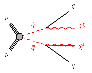
\includegraphics[width=\linewidth]{susy_standard}
    \caption{Event without initial state radiation~\cite{SUSYPub}.}
    \label{fig:susy_standard}
  \end{subfigure} \quad
  \begin{subfigure}[t]{.48\linewidth}
    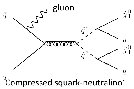
\includegraphics[width=\linewidth]{compressed}
    \caption{Event with initial state radiation~\cite{ExotPub}.}
    \label{fig:susy_compressed}
  \end{subfigure}
  \caption{Event topology of squark pair production resulting in a neutralinos
    with two jets final state with (\cref{fig:susy_compressed}) and without
    (\cref{fig:susy_standard}) initial state radiation.}
  \label{fig:motivation}
\end{figure}
\begin{figure}[!htb]
  \centering
  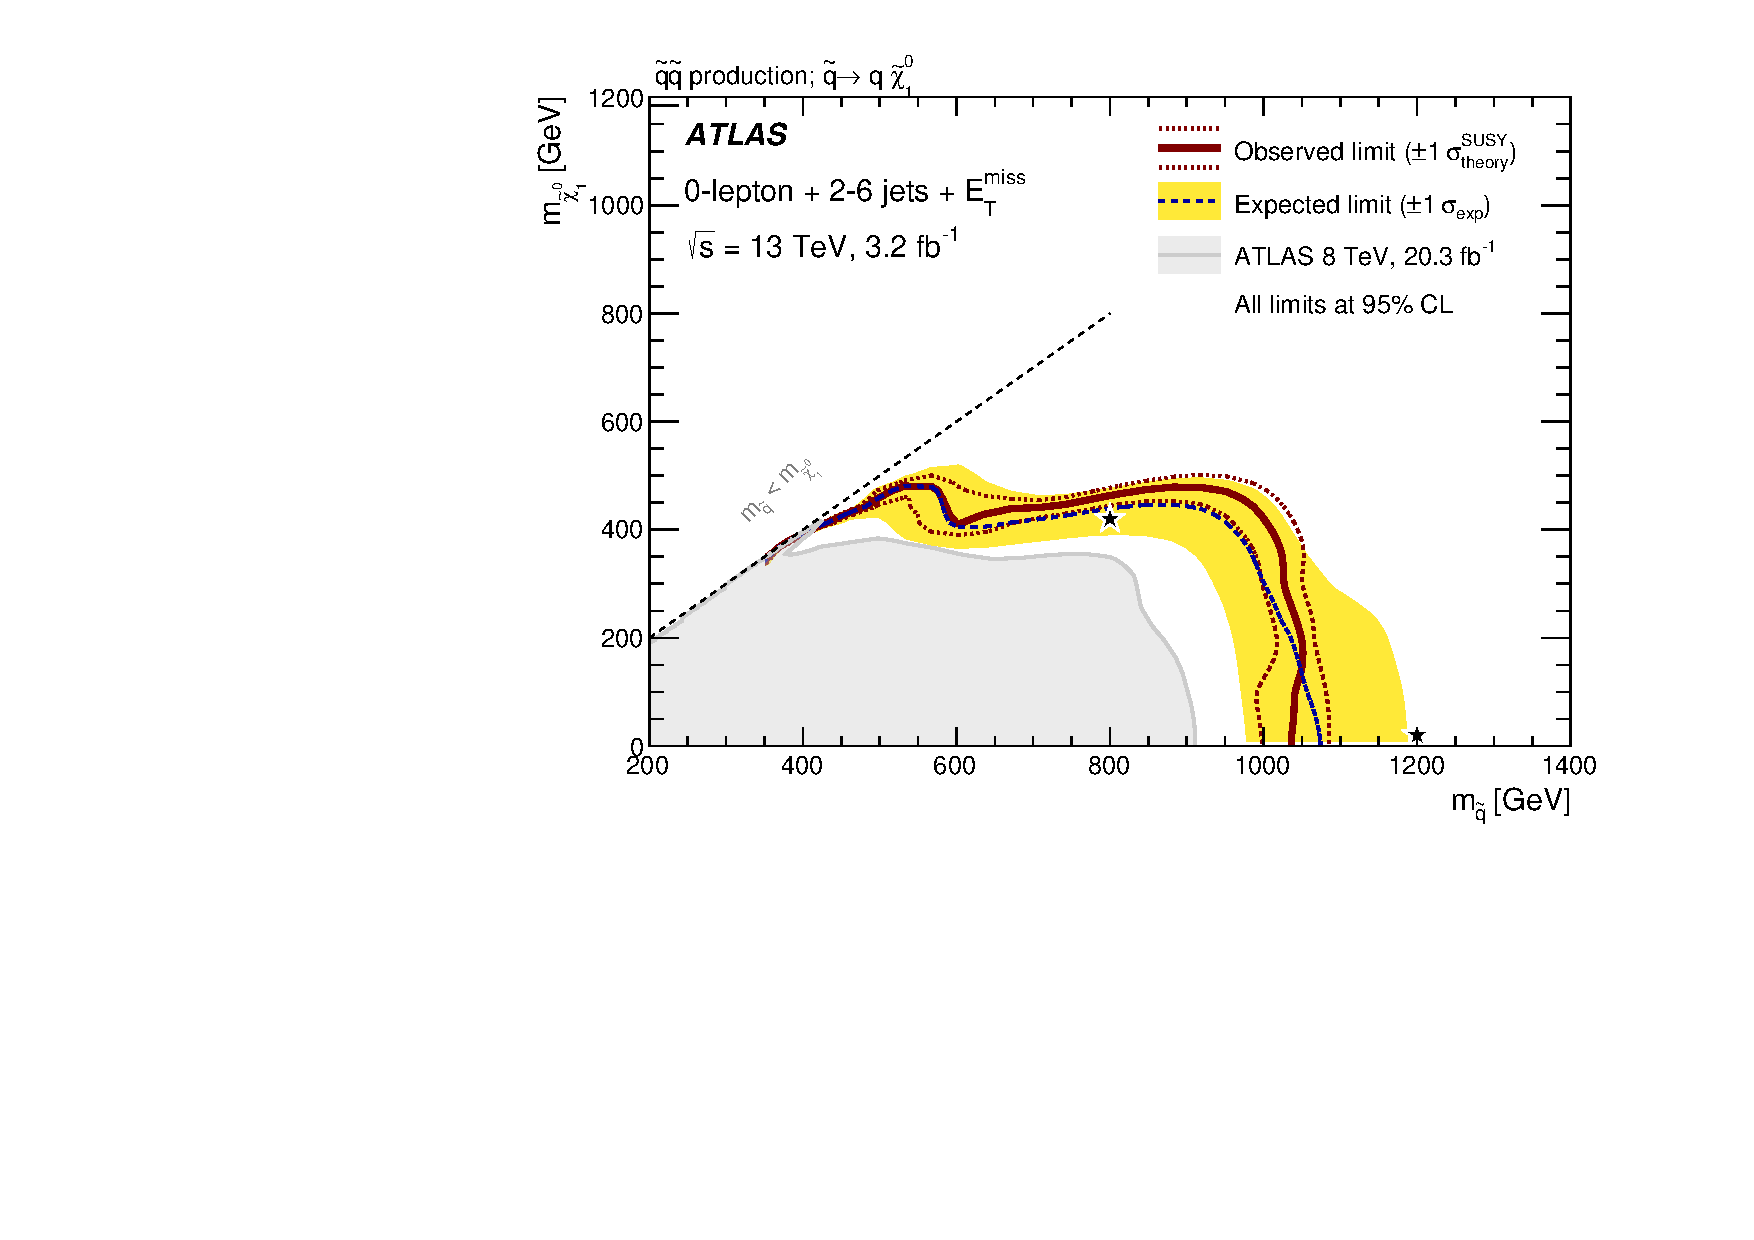
\includegraphics[width=.58\linewidth]{susy}
  \caption{Exclusion limits for direct production of squark
    pairs where the sqark decays into a quark and a neutralino. The $x$--axis
    represents the mass of the squark and the $y$--axis represents the mass of
    the lightest neutralino. The black stars represent a benchmark model as
    explained in more details in Ref.~~\cite{SUSYPub}.}
  \label{fig:susy_exclusion}
\end{figure}
%%% Local Variables:
%%% mode: latex
%%% TeX-master: "../search_for_DM_LED_with_ATLAS"
%%% End:


\section{Event Selection}
\label{sec:event-selection}

The search is carried out in $pp$ collisions using the data collected by the
ATLAS experiment during the 2015 Run II corresponding to a total integrated
luminosity of 3.2 \ifb.
%%% Local Variables:
%%% mode: latex
%%% TeX-master: "../search_for_DM_LED_with_ATLAS"
%%% End:


\begin{appendices}
  \chapter{Some title}
\end{appendices}

\addcontentsline{toc}{chapter}{\bibname} \printbibliography
\end{document}

%%% Local Variables:
%%% mode: latex
%%% TeX-master: t
%%% End:
